\chapter{项目设计}
\section{总体设计}
\begin{figure}[htbp]
    \centering
    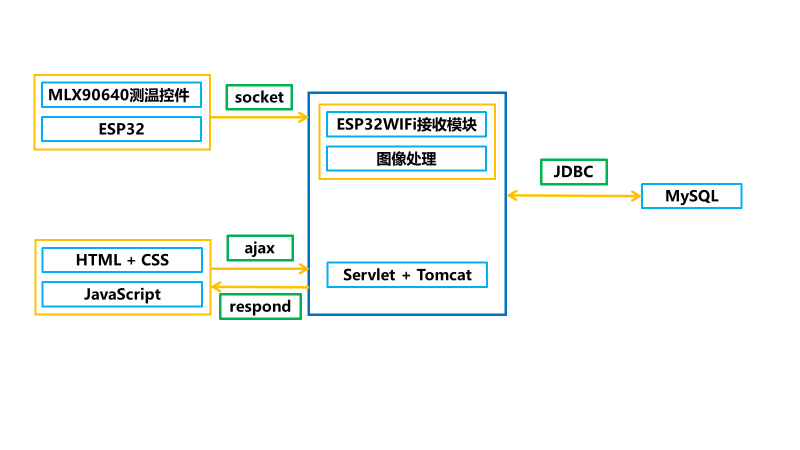
\includegraphics[width=0.8\textwidth]{design_1.png}
    \caption{总体设计}\label{fig:design_1}
    \vspace{\baselineskip}
    \end{figure}


\section{硬件系统设计}
(1)MLX90640温度采集模块

MLX90640 是工业标准并经过完全校准的 32*24
像素热红外阵列传感器,采用 4 脚 TO39 封装以及
I2C 兼容的数字接口。
MLX90640 包含 768 个热红外像素点。内嵌自身
环境温度传感器和 VDD 电压检测 ADC。通过 I2C 接
口,可以访问存储于内部 RAM 中的红外阵列、环境
温度以及 VDD 实时数据。

(2)ESP32模块
ESP32是一款安全稳定、低功耗、低成本的物联网芯片,搭载 RISC-V 32 位单核处理器,支持 2.4 GHz Wi-Fi 和 Bluetooth LE 5.0。为物联网产品提供行业领先的射频性能、完善的安全机制和丰富的内存资源。ESP32-C3 对 Wi-Fi 和 Bluetooth LE 5.0 的双重支持降低了设备配网难度,适用于广泛的物联网应用场景。

